%% PG-GAT architecture block diagram (fig:pggat_architecture).
%% Colour code: red = Mod 1 (type-pair bias), blue = Mod 2 (position encoding),
%% green = Mod 3 (repulsion heads). Matches the caption in chapter3_pg_gat.tex.
%% Build: pdflatex pggat_architecture.tex; output copied to ../pggat_architecture.pdf
\documentclass[10pt,tikz,border=6pt]{standalone}
\usepackage[T1]{fontenc}
\usepackage{mathptmx}
\usepackage{amsmath,amssymb}
\usetikzlibrary{positioning,fit,arrows.meta,calc}

\begin{document}
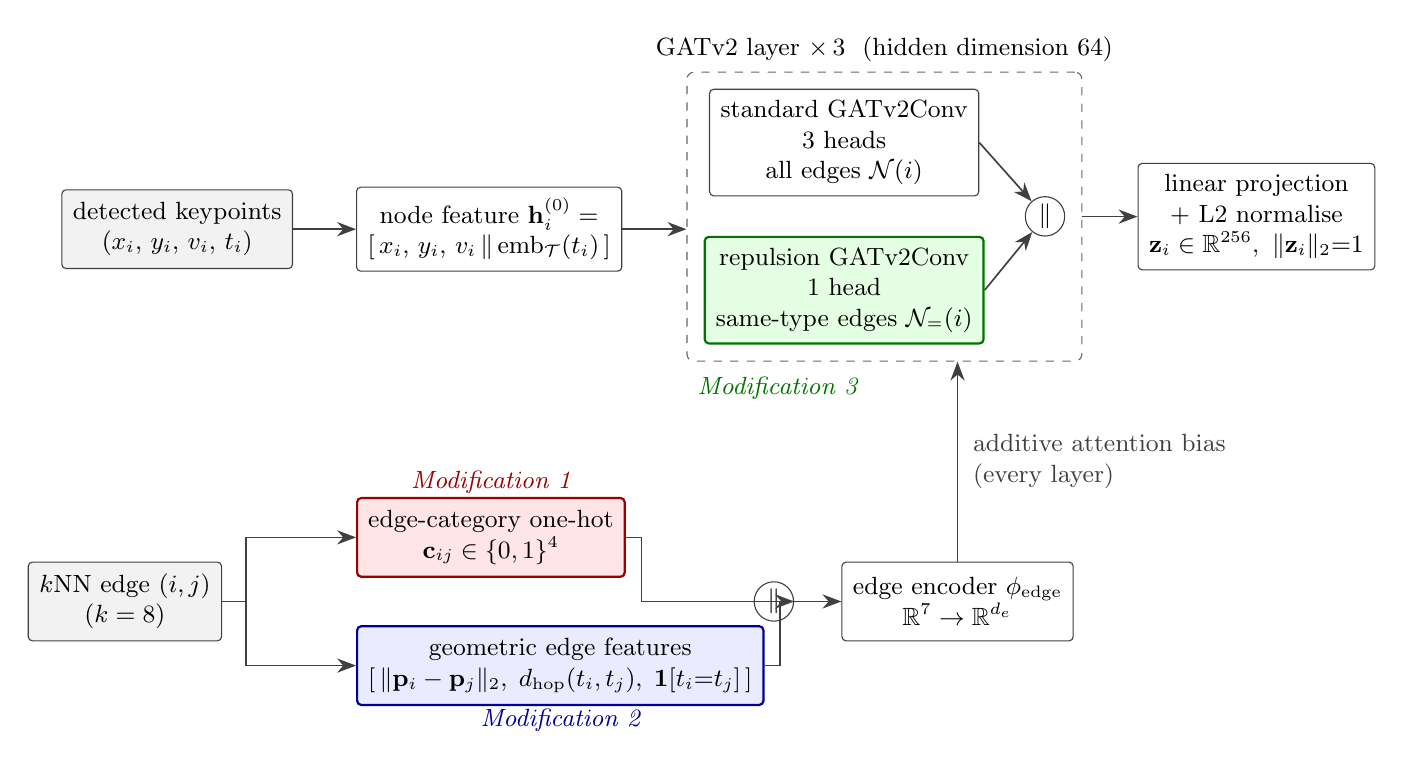
\begin{tikzpicture}[
  font=\small,
  >={Stealth[length=2.4mm]},
  box/.style={draw=black!75, rounded corners=1.5pt, align=center,
              inner sep=4pt, minimum height=10mm, fill=white},
  plain/.style={box, fill=black!5},
  mod1/.style={box, draw=red!60!black, fill=red!10, thick},
  mod2/.style={box, draw=blue!60!black, fill=blue!8, thick},
  mod3/.style={box, draw=green!45!black, fill=green!10, thick},
  cc/.style={circle, draw=black!75, inner sep=1.5pt, fill=white},
  arr/.style={->, semithick, black!75},
  modtag/.style={font=\small\itshape, inner sep=1pt},
]

%% ---------- node-feature path (top row) ----------
\node[plain] (kp) {detected keypoints\\ $(x_i,\, y_i,\, v_i,\, t_i)$};

\node[box, right=8mm of kp] (feat)
  {node feature $\mathbf{h}_i^{(0)} =$\\ $[\,x_i,\, y_i,\, v_i \,\|\, \mathrm{emb}_{\mathcal{T}}(t_i)\,]$};

%% GATv2 layer contents
\node[box, right=11mm of feat, yshift=11mm] (std)
  {standard GATv2Conv\\ $3$ heads\\ all edges $\mathcal{N}(i)$};
\node[mod3, below=5mm of std] (rep)
  {repulsion GATv2Conv\\ $1$ head\\ same-type edges $\mathcal{N}_{=}(i)$};
\node[cc] (headcat) at ($(std.east)!0.5!(rep.east) + (8mm,0)$) {$\|$};

\node[draw=black!60, dashed, rounded corners=2.5pt, inner sep=6pt,
      fit=(std)(rep)(headcat),
      label={[font=\small]above:{GATv2 layer $\times\,3$ \ (hidden dimension 64)}}]
  (gatbox) {};

\node[box, right=7mm of gatbox] (proj)
  {linear projection\\ $+$ L2 normalise\\ $\mathbf{z}_i \in \mathbb{R}^{256},\ \|\mathbf{z}_i\|_2{=}1$};

%% top-row arrows
\draw[arr] (kp) -- (feat);
\draw[arr] (feat.east) -- (gatbox.west |- feat.east);
\draw[arr] (std.east) -- (headcat);
\draw[arr] (rep.east) -- (headcat);
\draw[arr] (gatbox) -- (proj);

%% ---------- edge-feature path (bottom rows, mirrors the head split) ----------
\node[mod1, below=34mm of feat.west, anchor=north west,
      label={[modtag, red!60!black]above:{Modification 1}}] (cat)
  {edge-category one-hot\\ $\mathbf{c}_{ij} \in \{0,1\}^{4}$};

\node[mod2, label={[modtag, blue!60!black]below:{Modification 2}}]
  (geo) at ($(cat.south west) + (0,-6mm)$) [anchor=north west]
  {geometric edge features\\ $[\,\|\mathbf{p}_i - \mathbf{p}_j\|_2,\; d_{\mathrm{hop}}(t_i, t_j),\; \mathbf{1}[t_i{=}t_j]\,]$};

\node[plain] (knn) at ($(kp.south east |- cat.south) + (-9mm,-3mm)$) [anchor=east]
  {$k$NN edge $(i,j)$\\ ($k = 8$)};

\node[cc] (edgecat) at ($(cat.east)!0.5!(geo.east) + (10mm,0)$) {$\|$};

\node[box, right=6mm of edgecat] (enc)
  {edge encoder $\phi_{\mathrm{edge}}$\\ $\mathbb{R}^{7} \to \mathbb{R}^{d_e}$};

%% bottom-row arrows: knn feeds both feature constructors; both concat into the encoder
\draw[arr] (knn.east) -- ++(3mm,0) |- (cat.west);
\draw[arr] (knn.east) -- ++(3mm,0) |- (geo.west);
%% single junction so only one arrowhead meets the concat circle
\coordinate (ej) at ($(geo.east |- edgecat) + (2mm,0)$);
\draw[semithick, black!75] (cat.east) -- ++(2mm,0) |- (ej);
\draw[semithick, black!75] (geo.east) -- ++(2mm,0) |- (ej);
\draw[arr] (ej) -- (edgecat);
\draw[arr] (edgecat) -- (enc);

%% edge features enter the attention of every GAT layer
\draw[arr] (enc.north) -- (gatbox.south -| enc.north)
  node[pos=0.5, right=2pt, align=left, font=\small]{additive attention bias\\ (every layer)};

%% Modification 3 tag on the repulsion sub-layer (below the dashed container)
\node[modtag, green!45!black, anchor=north west] at ($(gatbox.south west)+(1mm,-1.5mm)$) {Modification 3};

\end{tikzpicture}
\end{document}
